\chapter{Method and materials}


\section{Study species} %Usikker på om eg skal ha med
%\subsubsection{Rev}  ?

%We also collated information on average body and home range sizes for a subset of species surveyed in the reviewed studies in order to better quantify the functional diversity of wildlife being sampled by CTs and to evaluate the degree to which CT methodologies were tailored to focal species. Burton 2015

The species I'll focus on in this thesis are the species that most frequently was observed \emph{(>50 events)}, excluding farmed animals (e.g. cattle), humans and dogs, and grouped categories of animals (e.g. birds).
Given that the decisions on cameras placement (height and angle) were made with photo capturing lynx() in mind, I have also excluded smaller species from the analysis.
This includes three species, squirrel(), hare() and European pine marten\textit{(Martes martes)}. 
Though they showed up frequently on many locations, there are inevitably some cameras that are too biased towards larger animals, resulting in an inconsistency of their detection rates. 
In turn, it is difficult to distinguish whether the species was affected by the white LED or not, as they could have triggered the camera, but already escaped the frame. %TODO må tygge litt på det argumentet.

In the end, the species I have used in my analyses are roe deer\textit{()}, red fox\textit{()}, badger\textit{(Meles meles)}, moose\textit{()}, red deer\textit{(Cervus elaphus)} and lynx. 

\section{Study area} %TODO 
%mogleg å kjøre ein fin overgang fra intro til study area? Study area valt pga dårlige snøforhold -> vanskelig å gjere spor-tellinger (\cite{Odden2015})


%https://klimaservicesenter.no/faces/desktop/article.xhtml?uri=klimaservicesenteret/klimaprofiler/klimaprofil-oslo-og-akershus
%https://klimaservicesenter.no/faces/desktop/article.xhtml?uri=klimaservicesenteret%2Fklimaprofiler%2Fklimaprofil-buskerud  
The study area (59.36-60.47° N, 9.43-10.91° E) %berre eit grovt overslag
extends over much of the southeastern parts of Norway in counties Flå, Krødsherad, Sigdal, Ringerike, Modum, Hole, Lier, Øvre Eiker, Asker, Oslo, Enebakk, Indre Østfold, Våler, Råde, Moss, Frogn and Vestby.
The climate has a continental character due to rain shadows of the mountain ridges from the west. 

The mean annual temperatures ranges from 2-6\celsius  and precipitation lies between 700-1500mm (\cite{Moen1999}). 
Topography is predominantly flat towards the south, and more rugged and elevated towards the north. The landscape is a mosaic of forest and agricultural areas, divided with a wide network of gravel roads.
The area is situated in the southern boreal and the boreonemoral zones. %Må finne oppdaterte data (frå Norges vassdrags- og energidirektorat, 2019?)

Norway spruce (\textit{Picea abies}) and Scots pine (\textit{Pinus sylvestris}) make up the dominating boreal coniferous forests, with frequent presence of silver birch (\textit{Betula pendula}) and downy birch (\textit{Betula pubescens}), then aspen (\textit{Populous tremula}), alder (\textit{Alnus incana}) and black alder (\textit{Alnus glutinosa}).

Growing season length 170 - 190 days (Moen, 1999, map 6, s.21) %må finne oppdaterte data
Snow cover length												%må finne oppdaterte data

Most cameras were set in forest areas, usually by a tractor path or human trail, sometimes by animal paths. Their distance from houses or roads varied to a large extent, and some areas were logged (ved Vansjø) and even greatly changed under development of new infrastructure (toglinje på nordligste kamera ~1255)


\section{Study design} %TODO
For the study I chose 60 already established camera sites with infrared light(Reconyx and Browning models), in order to have a reference of capture frequencies. The cameras had been installed on trees 1-3 meters from human or tractor paths, 40-120 cm above ground level, with the original aim to photo capture lynx (\cite{Odden2015}). 
I divided the sites randomly into three groups of 20 cameras. Cameras in group A remained unchanged, whilst group B and C were equipped with an additional white LED camera (Reconyx PC850) in alternating 3 month-periods, as shown in figure\vref{fig:exp_set}.

\begin{figure}
    \begin{center}
    	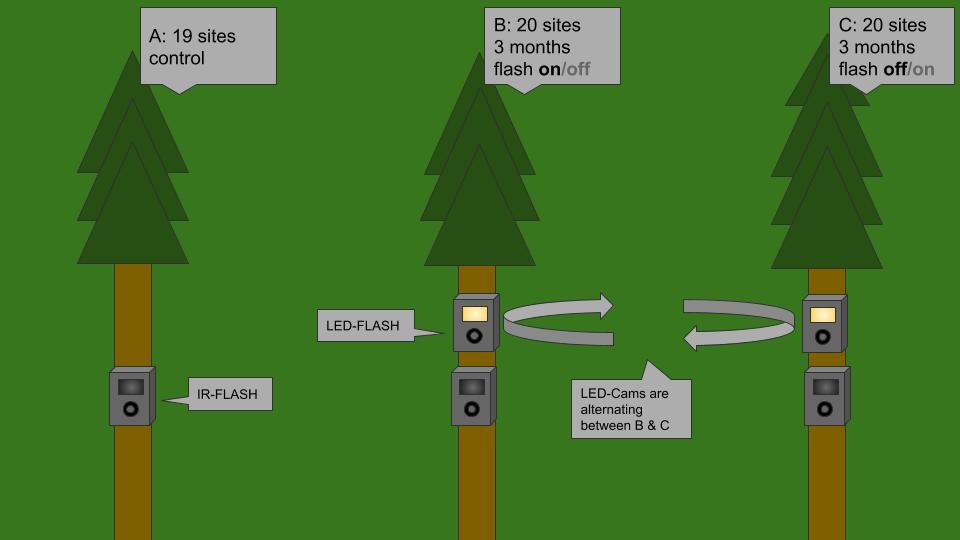
\includegraphics[scale=0.3]{experiment_setup} %insert figure of groups     
    \end{center}
    	\caption{Experiment setup}
    \label{fig:exp_set}
\end{figure}


The preinstalled cameras were set up and handled by people from the Norwegian Institute of Nature Research (NINA) and --- at the sites further from Oslo  --- by members of the Norwegian Hunters and Fishers Society (NJFF). 
%as a conflict mitigating strategy. %%Kan kuttes. Evt må det forklares
Thus, the installation of the cameras did not follow a strict protocol, nor were their locations chosen randomly. The overall placement was systematic as decided by NINA, then there was a deliberately-biased placement of the CTs put up in areas where the individual handler deemed it most likely to photograph lynx,
and hence, based on a combination of site accessibility and expectations of animal occurence (\cite{Burton2015}). %TODO vask språket 

%\emph{presence of natural or artificial attractants may draw animals in to a CT} \cite{Burton2015}.

As shown in figure\vref{fig:exp_set}, I set up all white LED cameras above the cameras already in place. 
However, at the particular site shown in figure\vref{fig:cam_ex_c} the infrared camera had been installed so far above ground level that I chose to position the white LED camera below the camera already in place. %endra på av Atle, men kan vaskas ytterligere 
For the periods without white flash treatment, I moved the cameras to their next site. However, the boxes installed on the trees remained (see figure \ref{fig:cam_ex_d}).
First, I equipped Group B with white LED in a 3 week period from January - February 2019. The boxes remained untill the end of the experiment. Group C, on the other hand, had no extra boxes before the start of the second period in May 2019 (i.e. remained identical to the control group A untill May).


I visited sites of group B and C at least once every three months in order to move the LED cameras. For convenience I visited sites of group A less often. %Her trengs ein språkleg endring
However, as the cameras were part of other, ongoing projects, they were occasionally visited by other workers from NINA to retreive the Secure Digital memory cards (hereby SD Cards) for data. %write in full on first mention (-Atle)
This was mostly the case for sites close to, and south of, Oslo, or rather, the cameras not normally operated by members of the NJFF.



\begin{figure}
		\begin{subfigure}{.5\textwidth}
		  \centering
		  	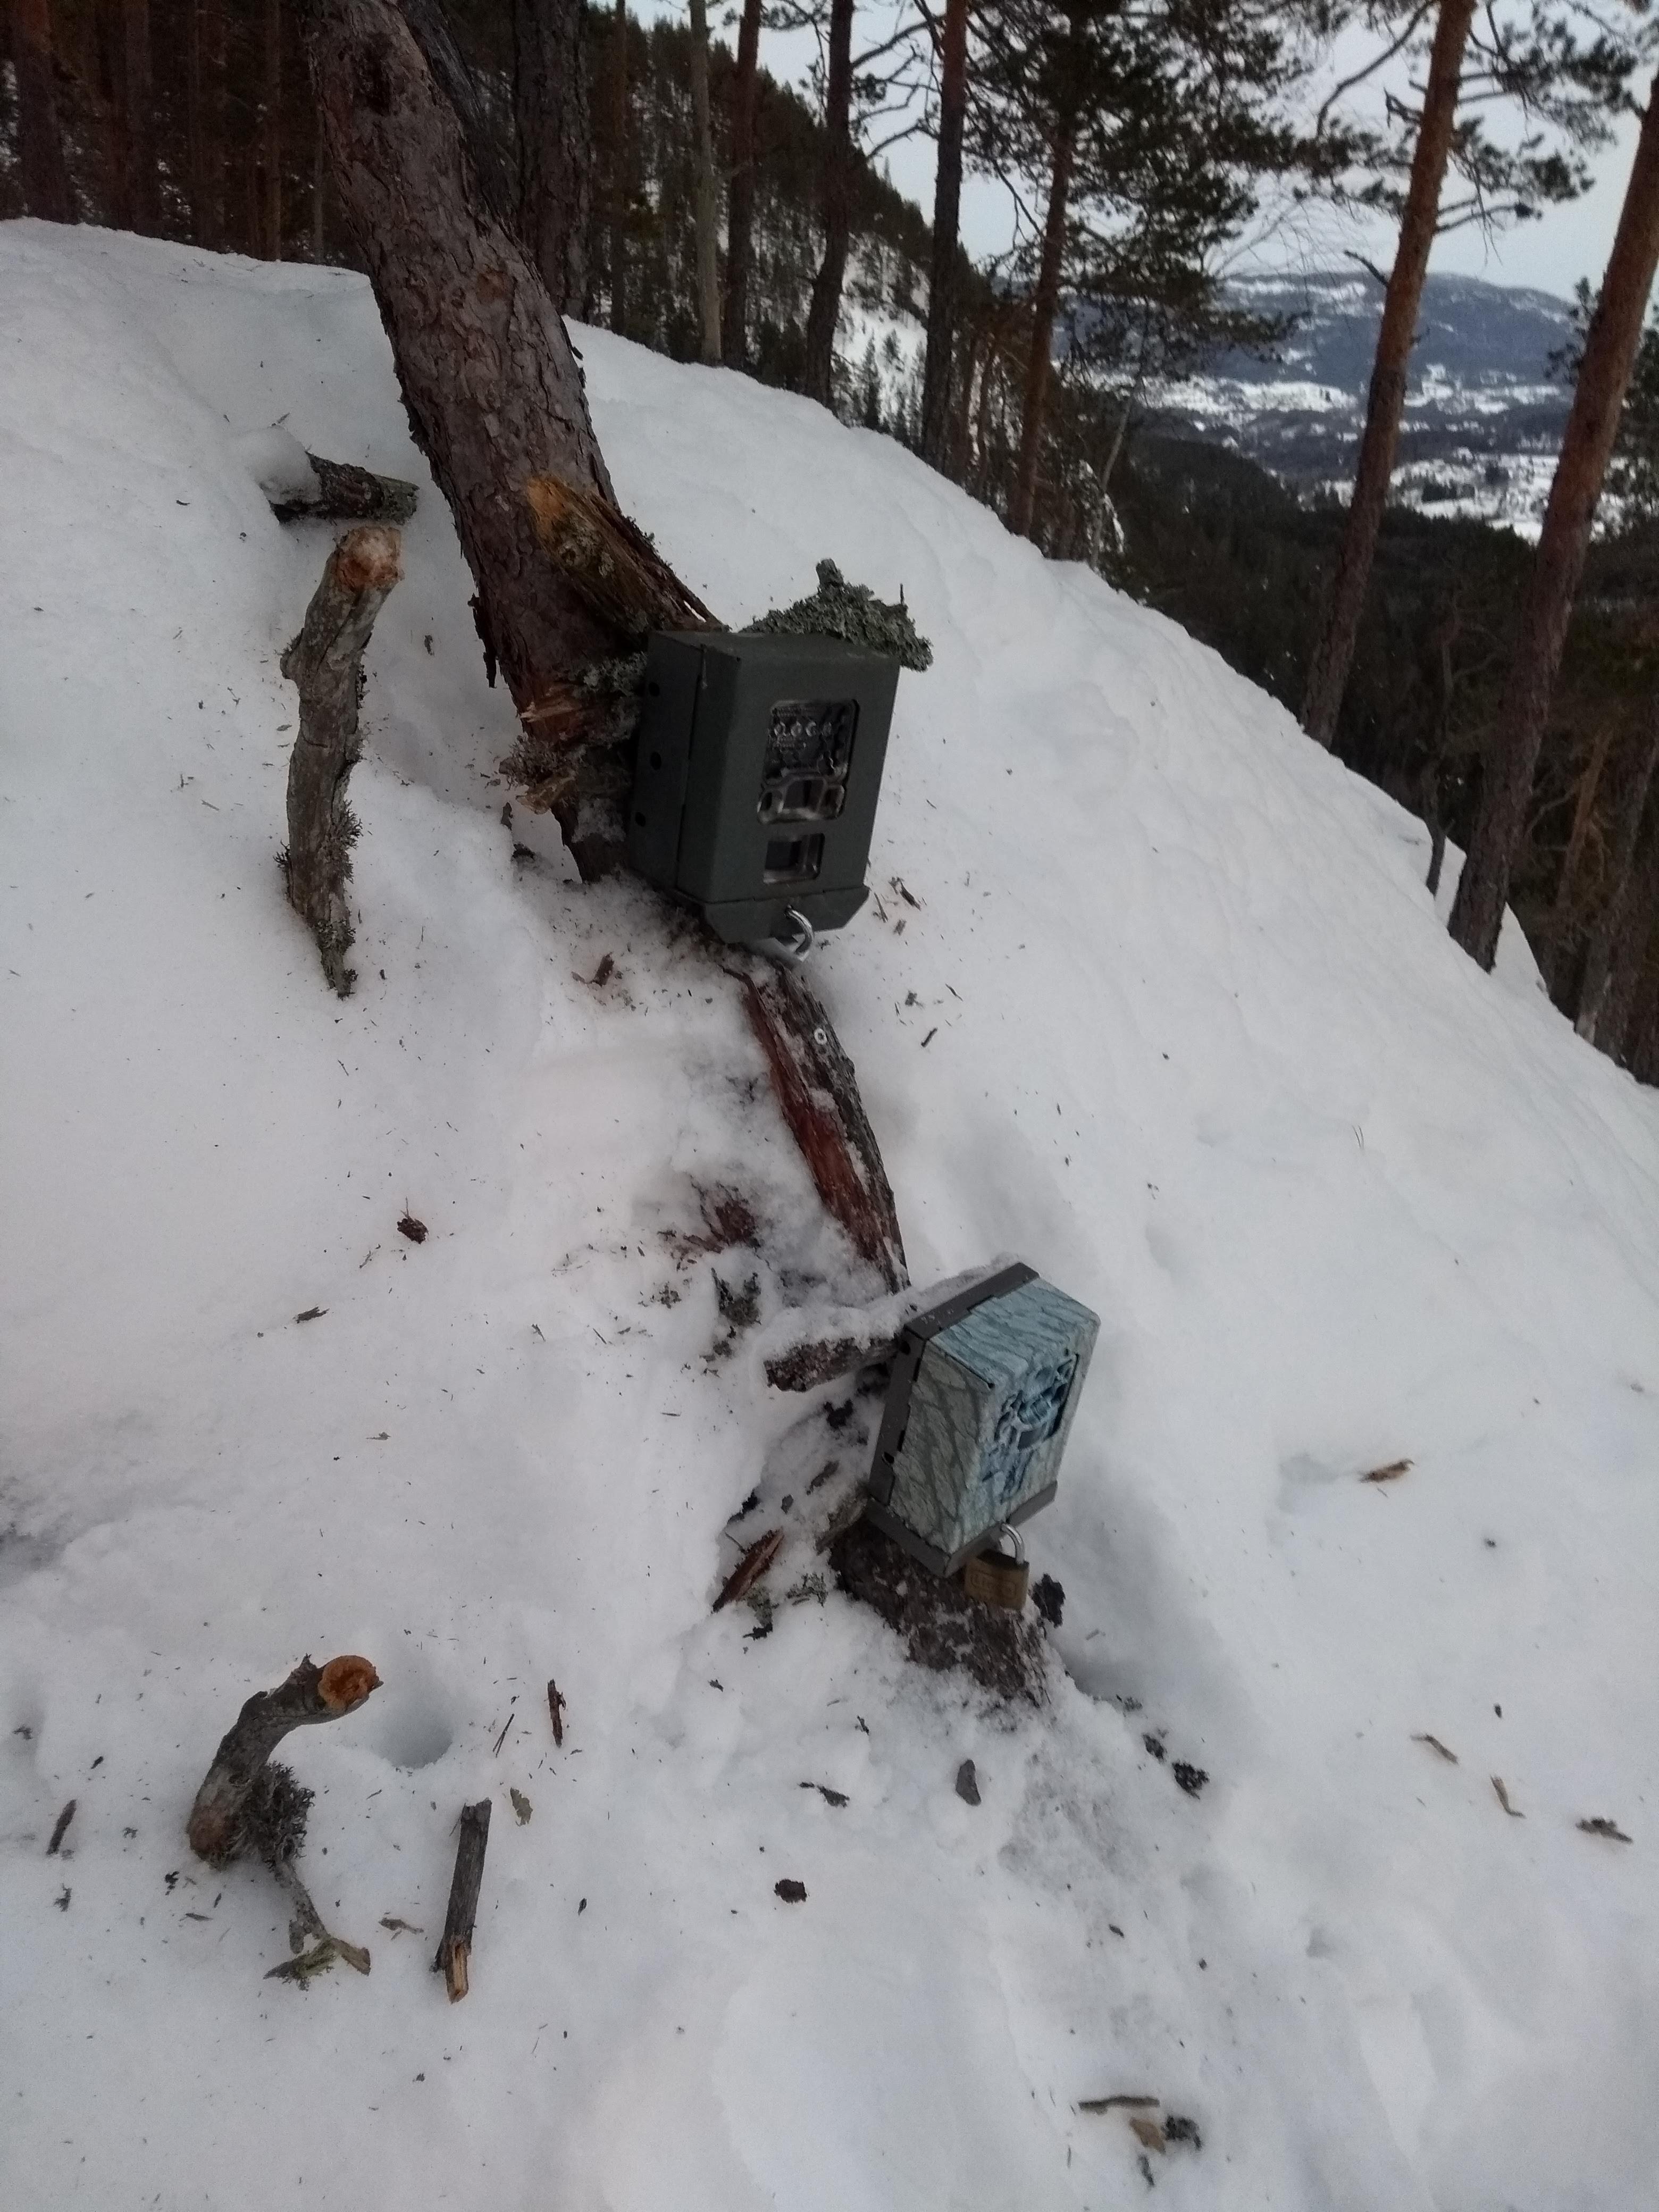
\includegraphics[width=.8\linewidth]{/cam_install_example/IMG_20190212_161615169}
		  \caption{Browning infrared,\\ installed on a fallen tree}
		  	\label{fig:cam_ex_a}
	\end{subfigure}
		\begin{subfigure}{.5\textwidth}
		  \centering
		  	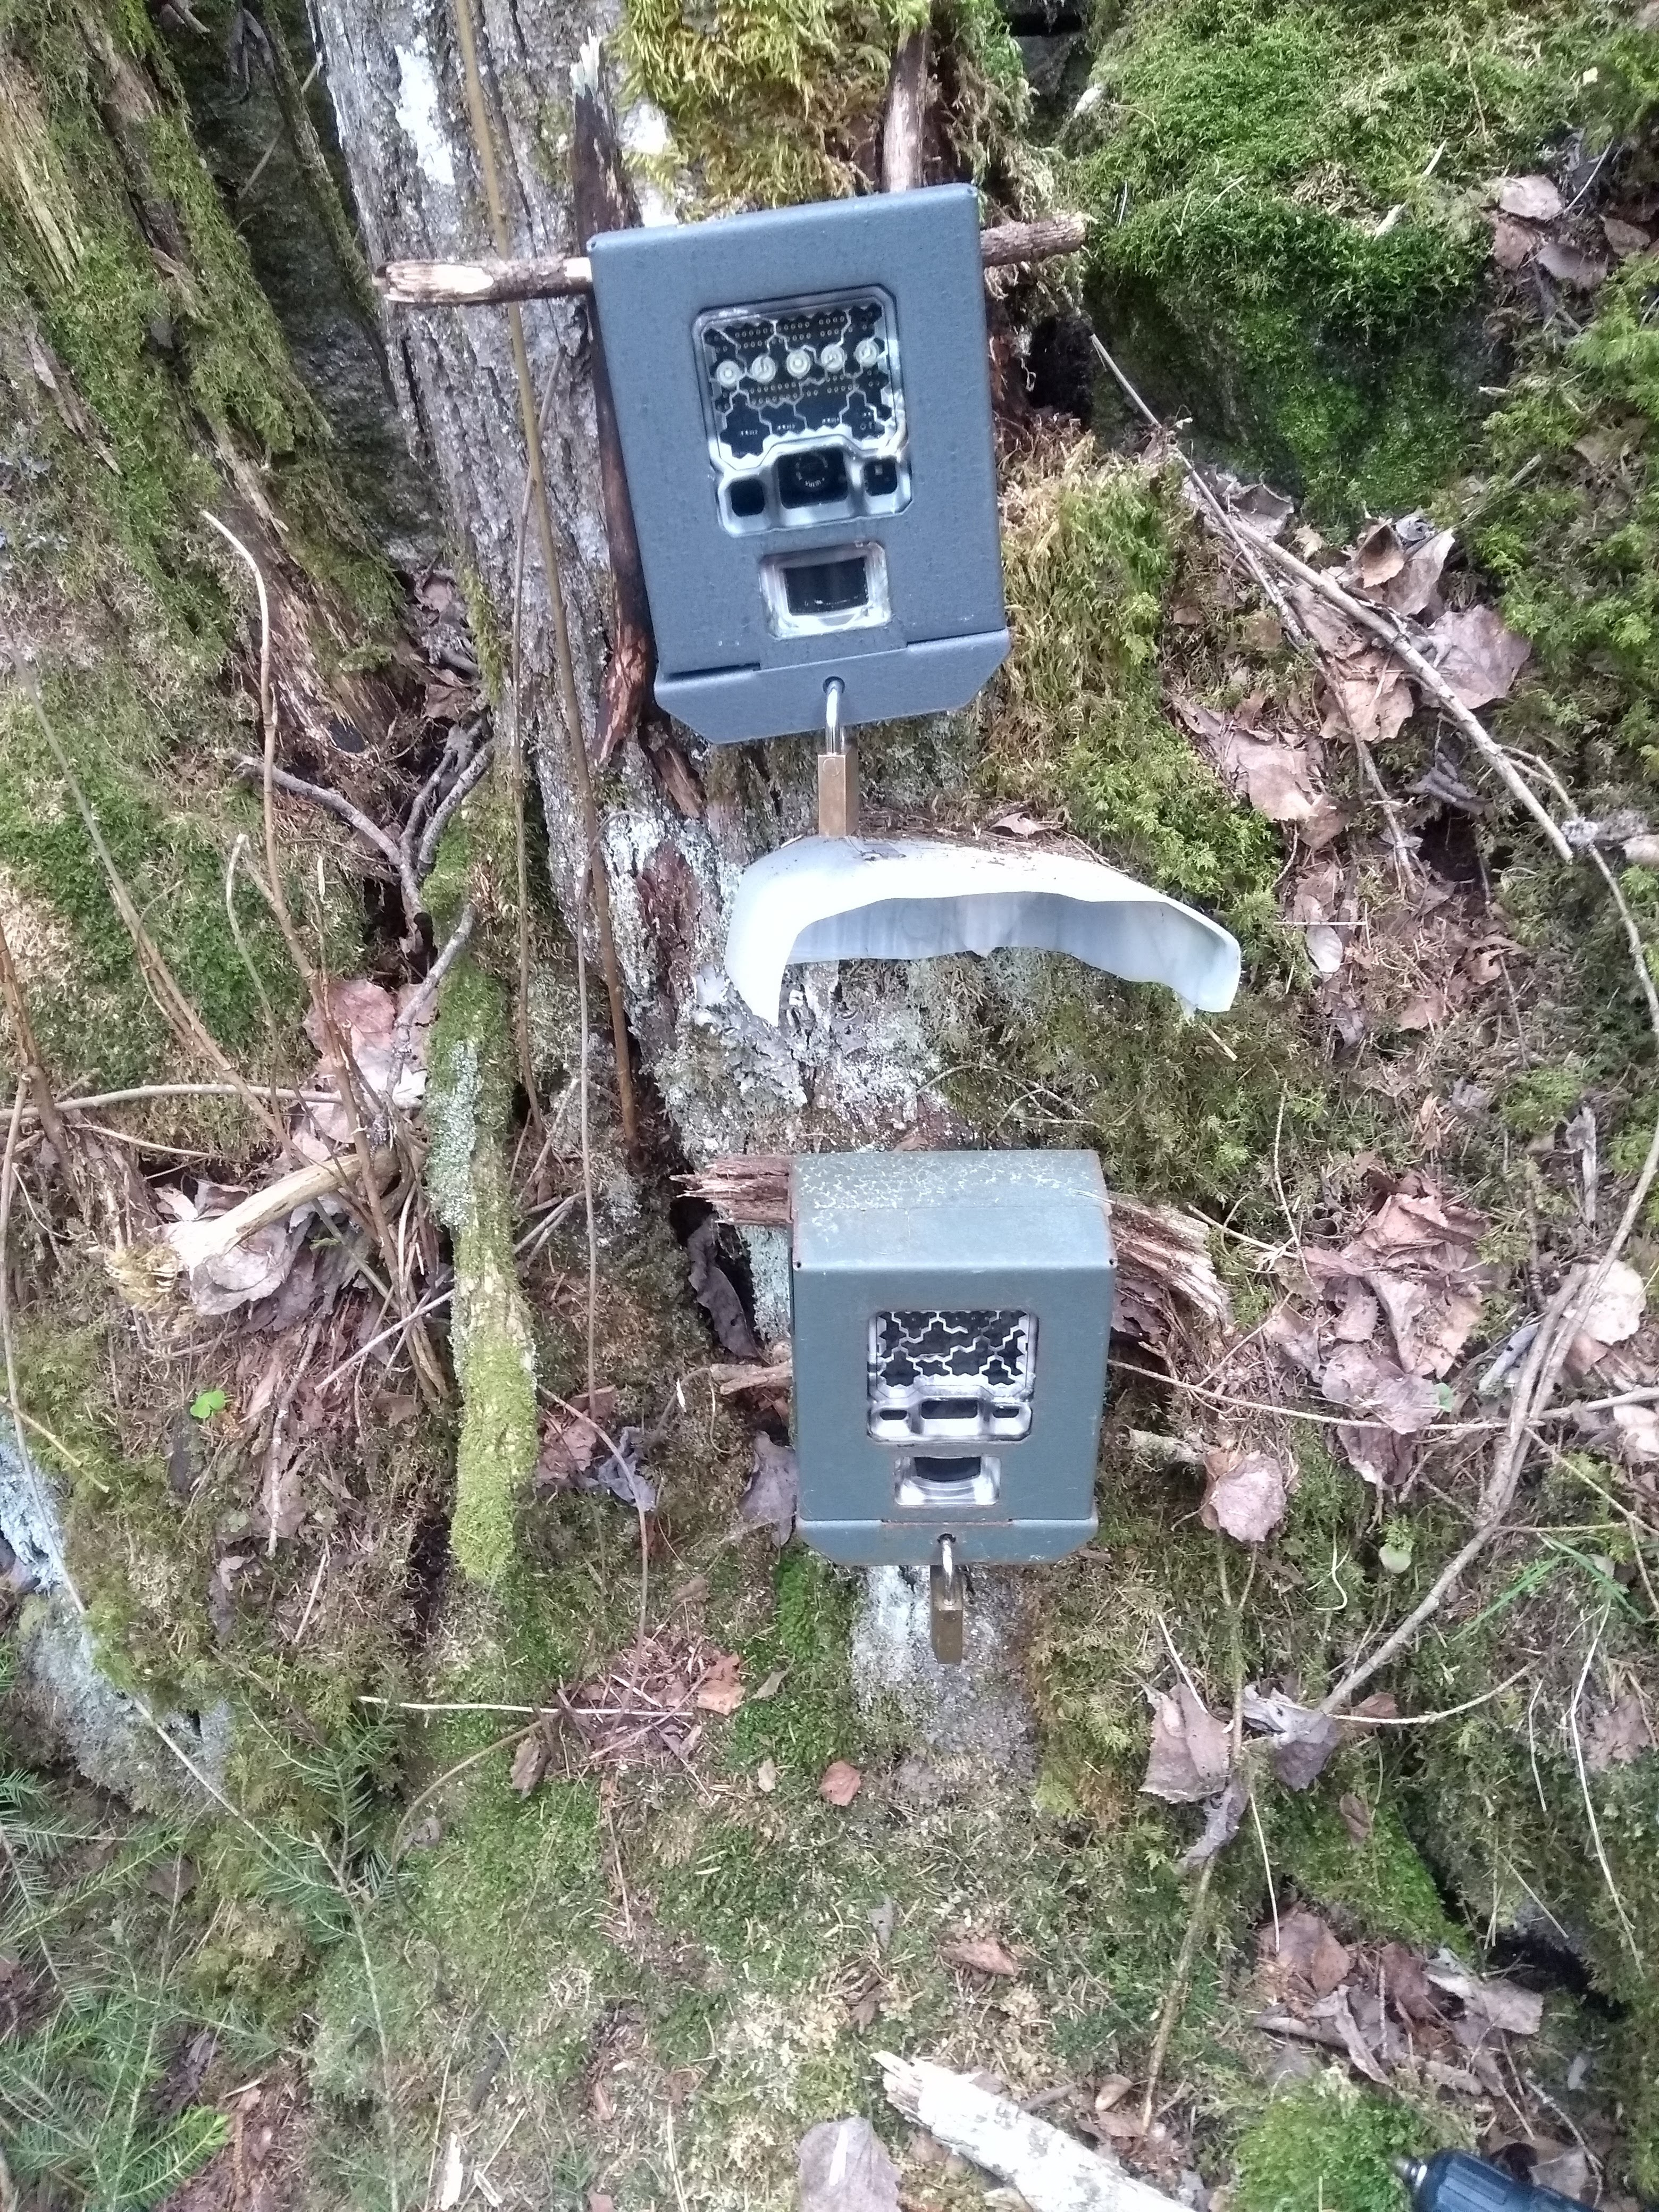
\includegraphics[width=.8\linewidth]{/cam_install_example/IMG_20190515_170952923}
		  \caption{Reconyx infrared,\\ installed with a snow cap}
		  	\label{fig:cam_ex_b}
	\end{subfigure}
		\begin{subfigure}{.5\textwidth}
		  \centering
		  	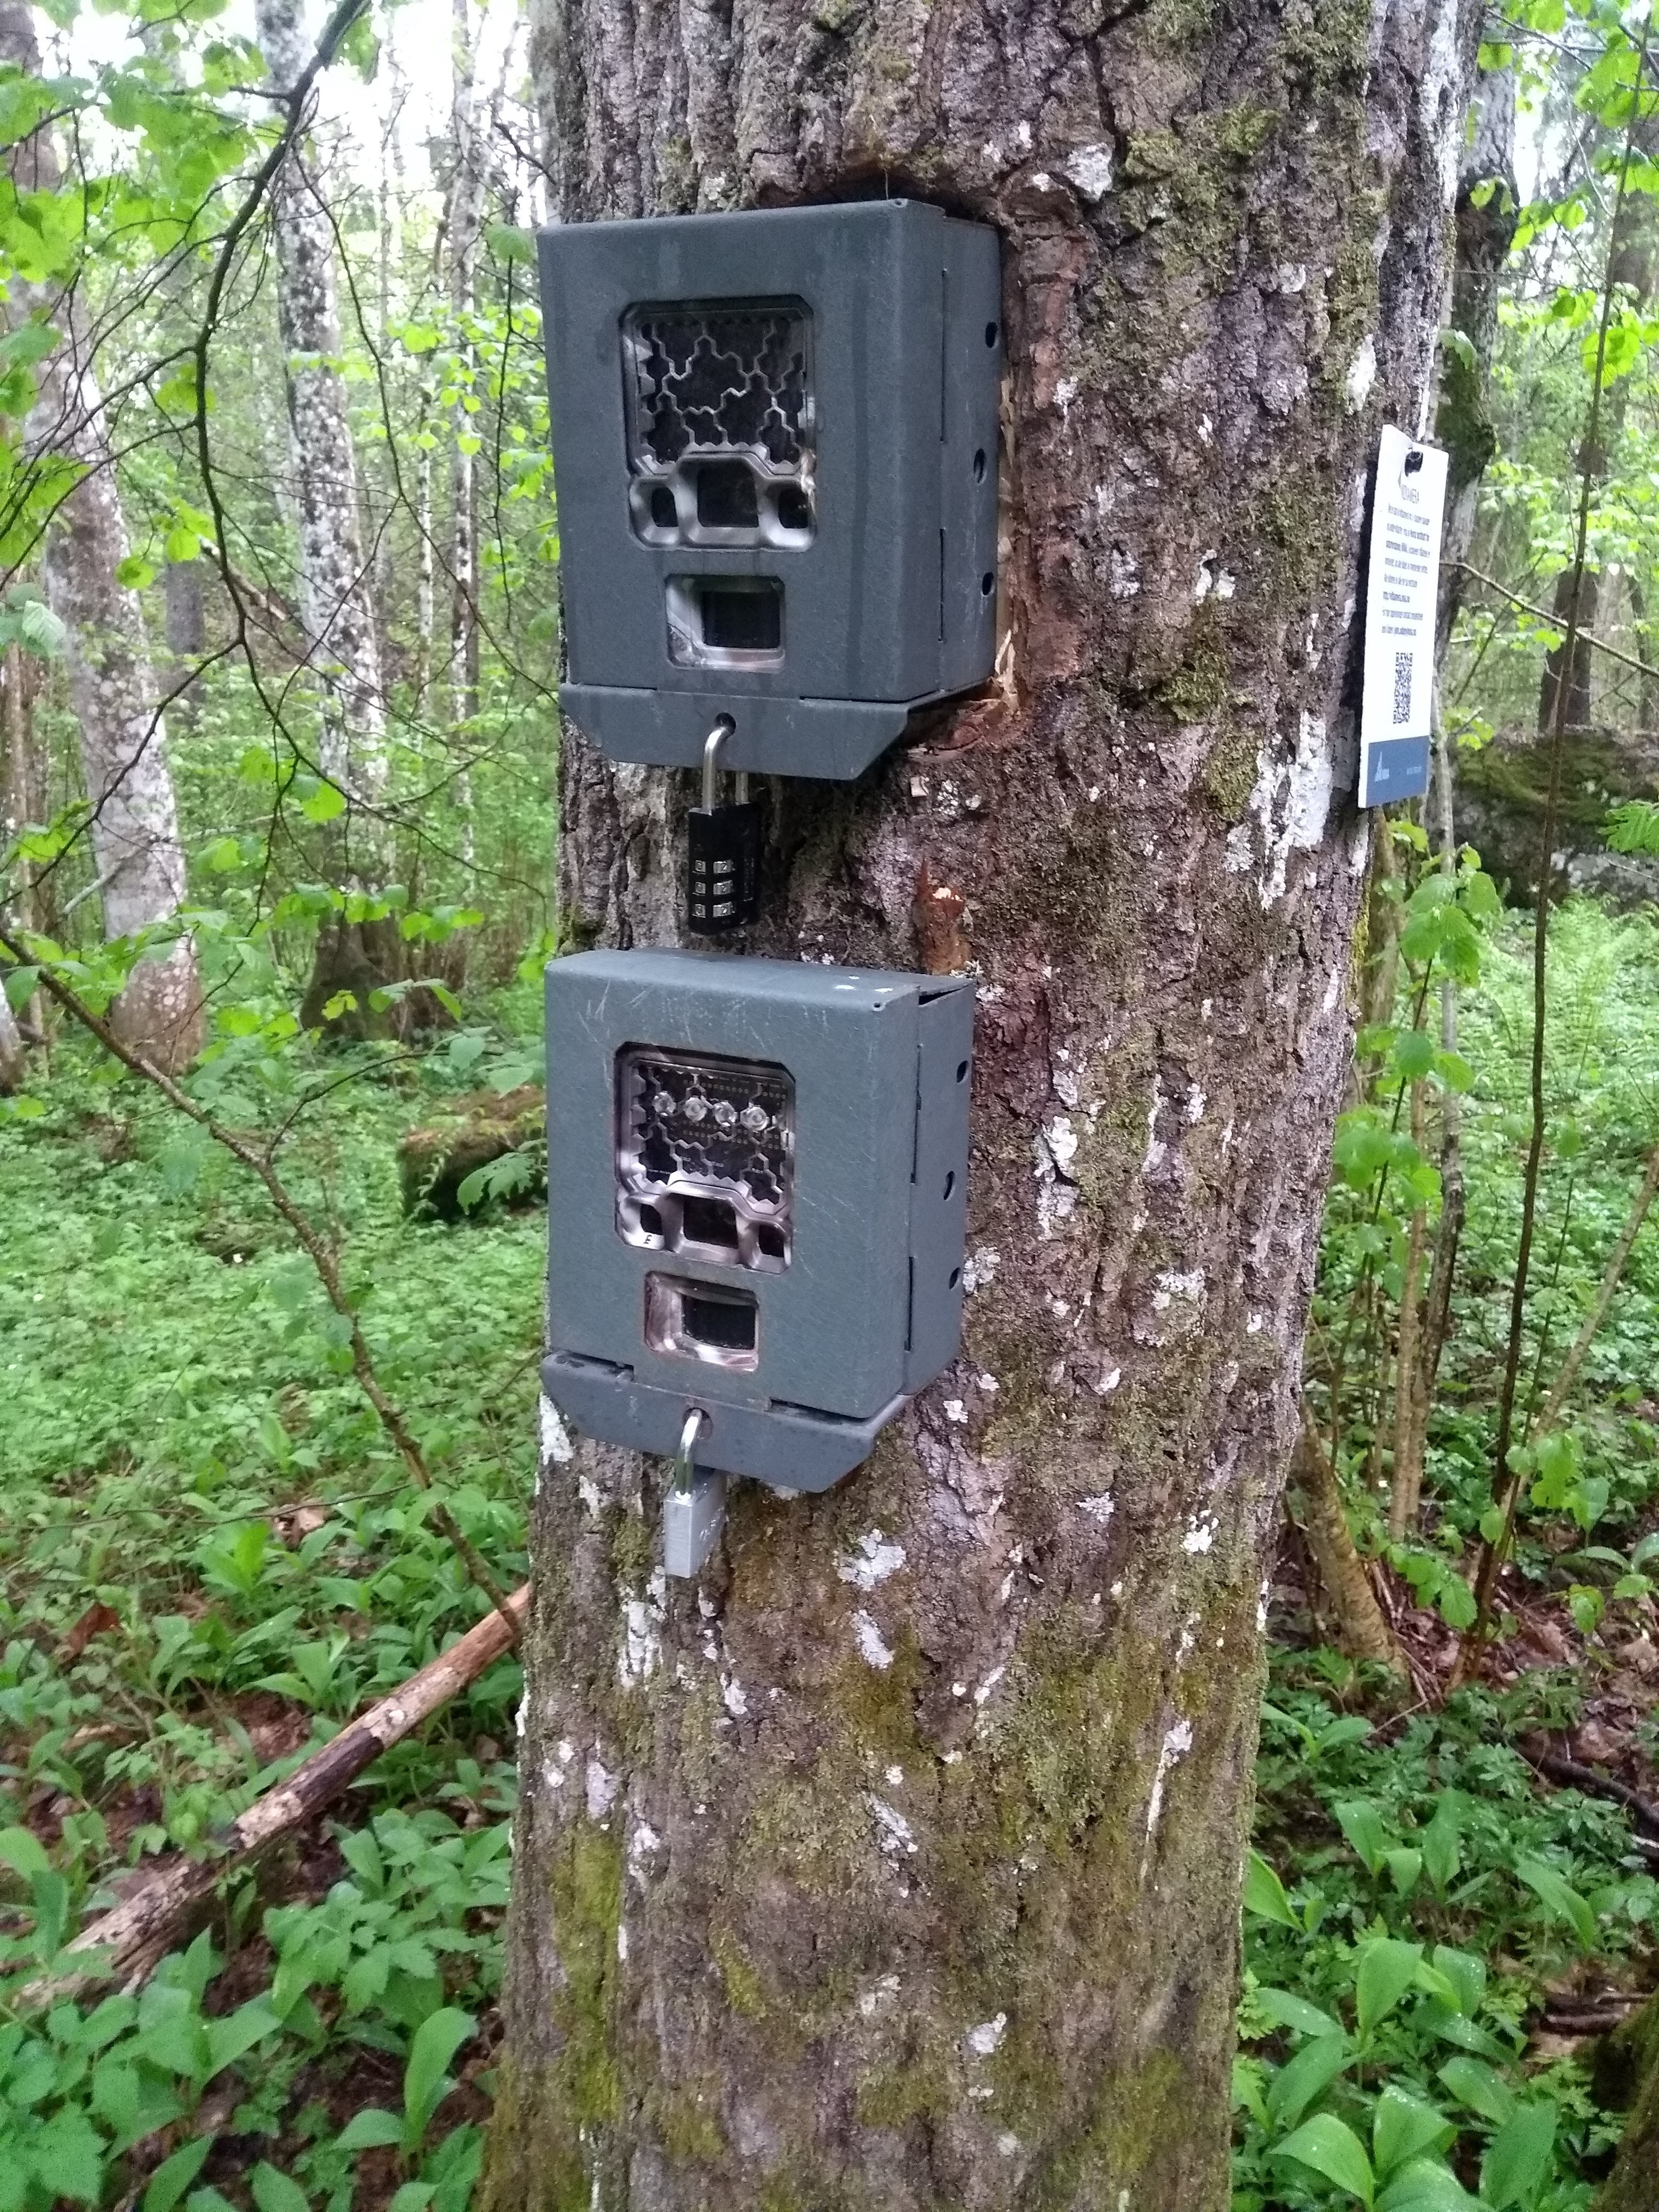
\includegraphics[width=.8\linewidth]{/cam_install_example/IMG_20190521_181329313}
		  \caption{Reconyx infrared above,\\ installed 160 cm above ground level}
		  	\label{fig:cam_ex_c}
	\end{subfigure}
		\begin{subfigure}{.5\textwidth}
		  \centering
		  	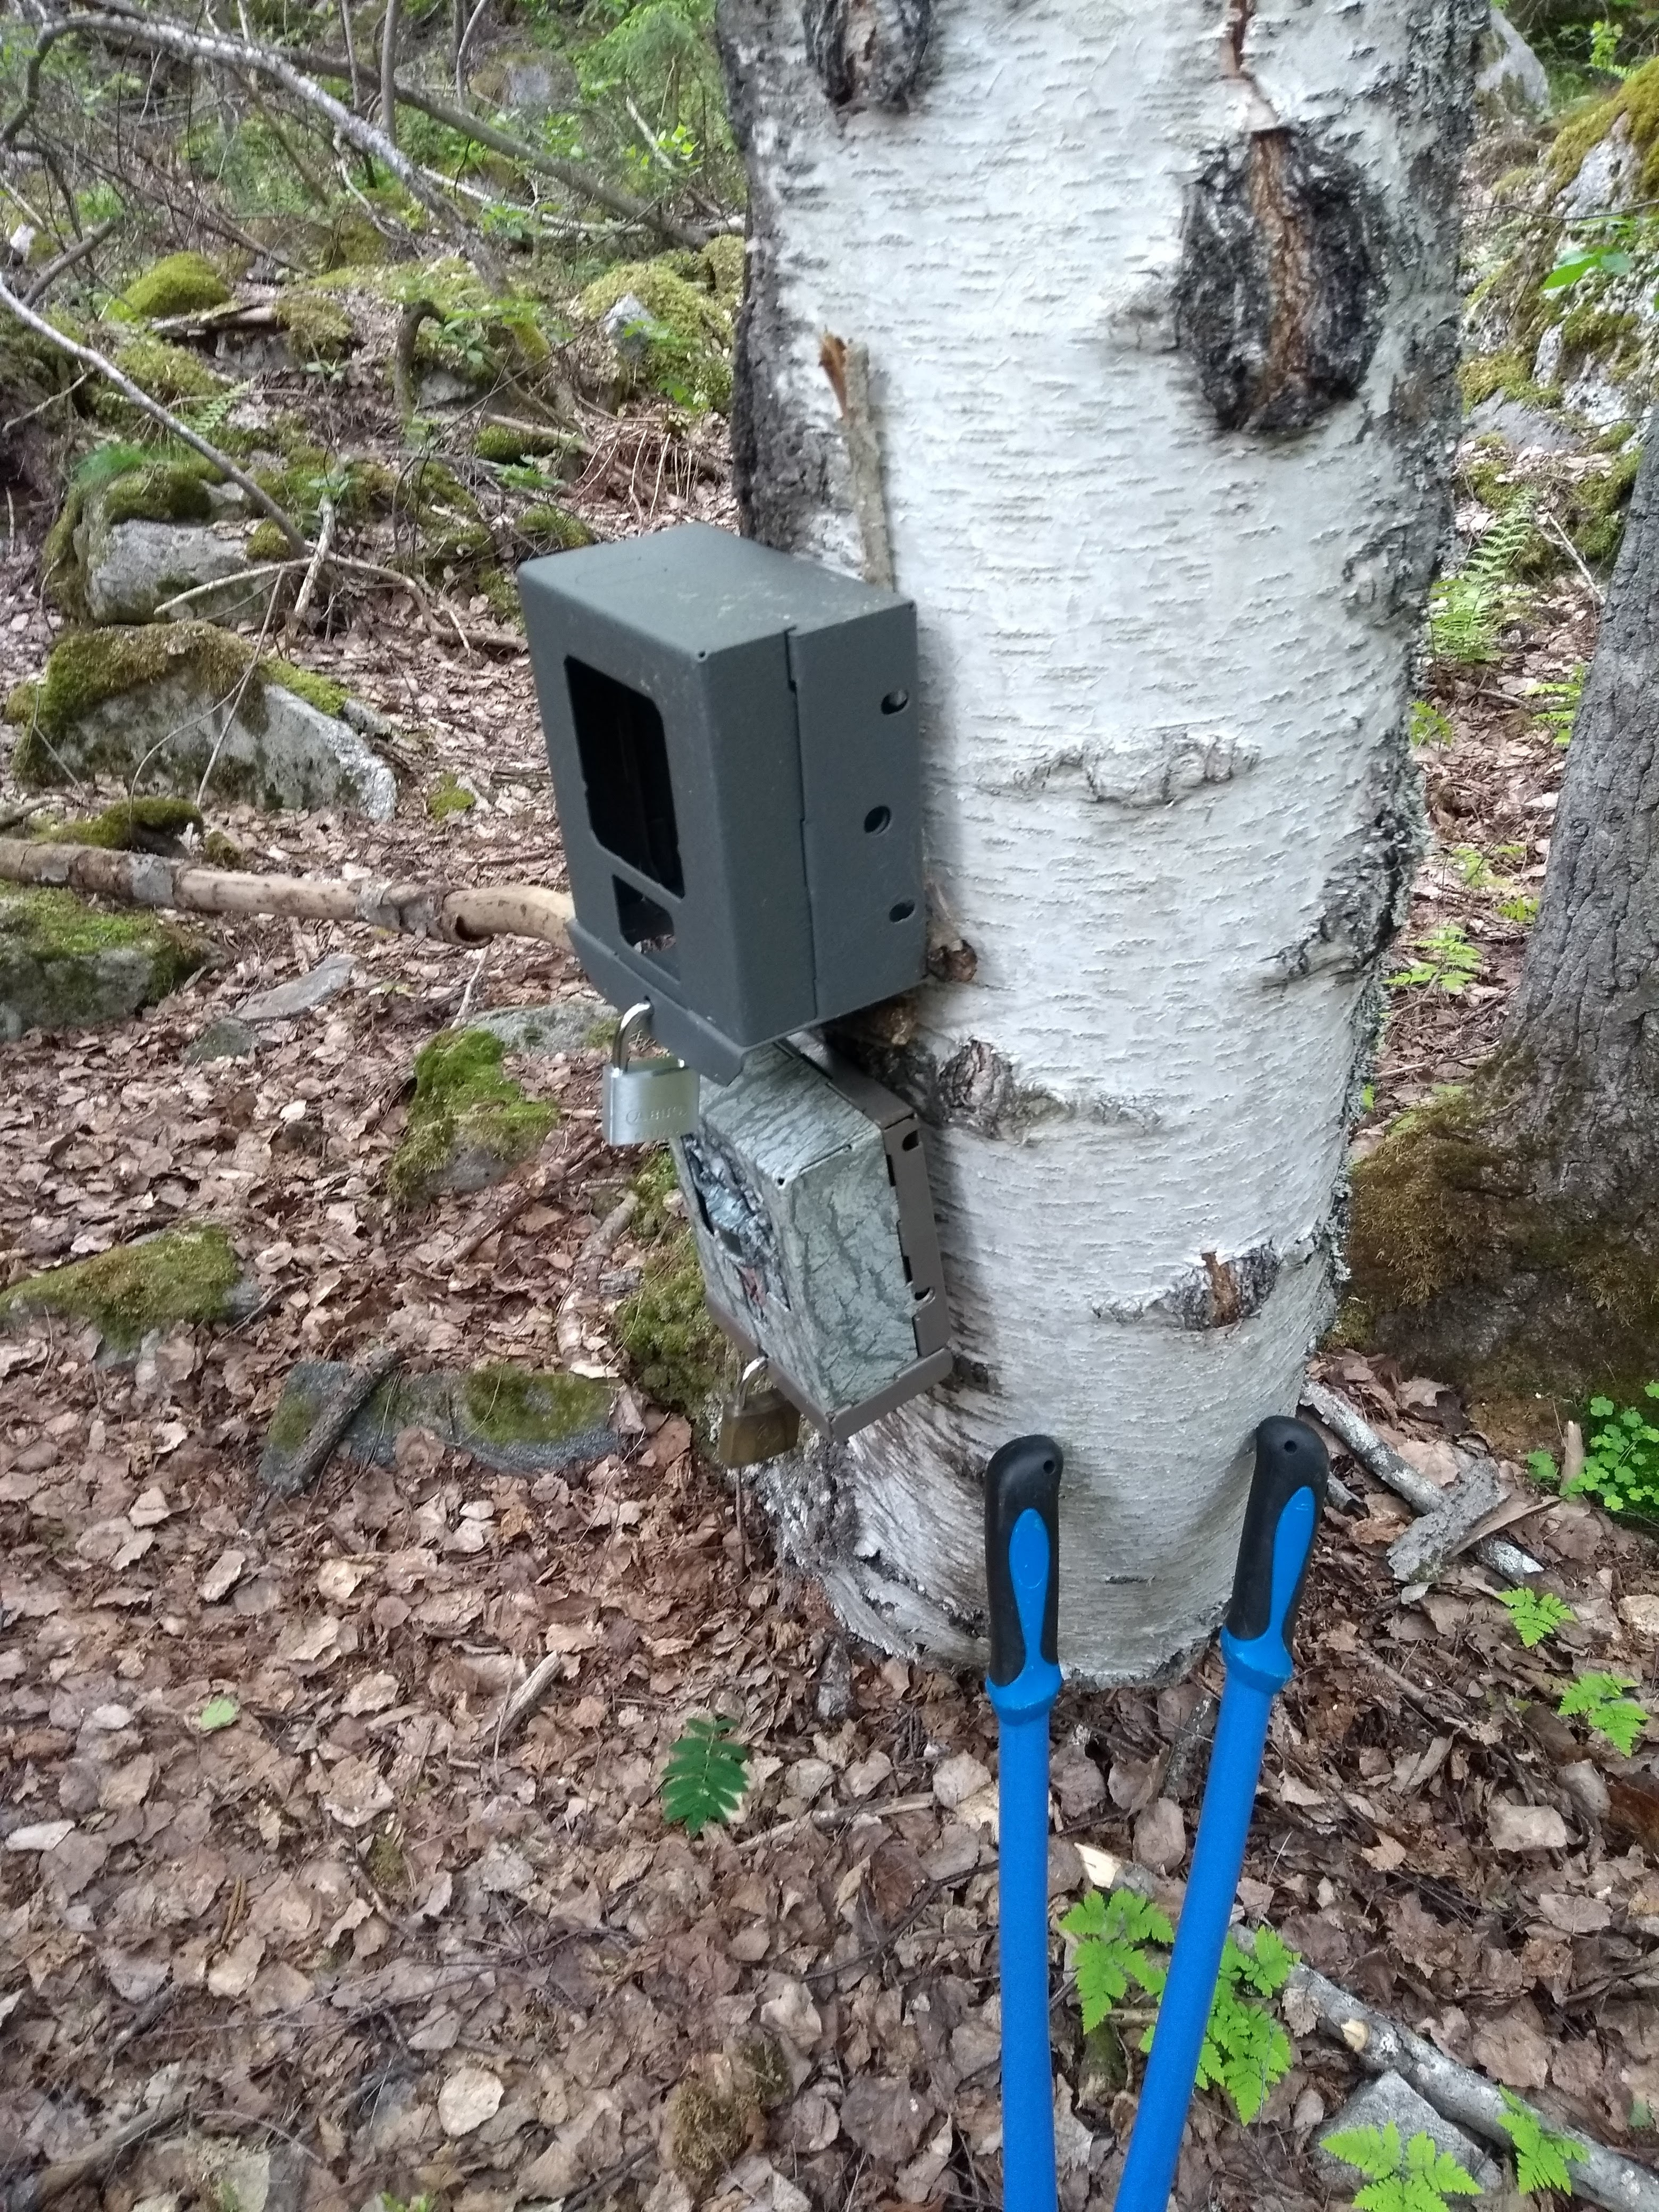
\includegraphics[width=.8\linewidth]{/cam_install_example/IMG_20190529_181049340}
		  \caption{Browning infrared,\\ white LED flash has just been removed}
		  	\label{fig:cam_ex_d}
	\end{subfigure}
		\caption{The preinstalled cameras varied in the way they were set up. Lower cameras with infrared, upper cameras with white LED (except in example c)}
	\label{fig:cam_ex_main}
\end{figure}

%We quantified the degree of consistency in implementing and reporting features of CT protocols and study design that might affect detectability and sampling error (e.g. camera type and settings, spatial and temporal sampling effort, use of attractants; Table S1). These details are fundamental to interpreting results of CT studies and assessing their reliability, repeatability and suitability for broader comparison or synthesis (Meek et al. 2014a)

%TODO Details of camera trap orientation, use of lures, and performance settings are also critical elements of camera trapping methodology. The height in relation to the target, the direction the camera is facing in relation to expected animal travel and path of the sun as well as horizontal and vertical alignment may all influence the results of camera trap studies. Providing clear descriptions of exactly how cameras were placed is fundamental to understanding and interpreting the results of research. (Meek etal 2014)


\section{Data Collection} %TODO  Trenger kilde på AI! 
%The fieldwork was conducted between September 15 and December 20, 2017. In this study, camera traps from the Norwegian Institute for Nature Research (NINA) were used. NINA uses camera traps to monitor the Eurasian lynx in southeastern Norway as part of the SCANDLYNX project (Odden, 2015). SCANDLYNX is a Scandinavian research project on the Eurasian lynx (Odden, 2015; SCANDLYNX, 2017). Camera traps were placed specifically with the goal to photo-capture lynx, and were therefore placed in steep terrain, on ledges or facing the cliff bases, often close to wildlife trails. The cameras were pointing perpendicular to the wildlife trail at locations where a wildlife trail was present. Each camera was mounted on a tree between 0.2 and 1 m above ground

Five different models of RECONYX™ (address: 3828 Creekside Ln, Ste 2, Holmen, WI 54636, USA, www.reconyx.com) cameras were used, 
and one model of BROWNING™ (address: One Browning Place, Morgan, UT 84050, USA, www.browningtrailcameras.com) \ref{tab:cam_mod}.

Reconyx-cameras have been reported of having an average trigger speed of 0.2 seconds, whereas the Browning model was reported an average of 0.7 seconds (Trigger speed shootout, \cite{Trailcampro2014}).


\begin{table}
\caption{\label{tab:cam_mod} Camera models}
\centering

\begin{tabular}{llrrr}
\hline
Producent  & Model name & Flash type & Trigger speed & N \\
\cline{1-2}
\multirow{5}{2cm}{Reconyx HyperFire Series} &
	  HC500 Semi-Covert IR					& IR	& 0.2s &  ? \\
	& HC600 High-Output Covert IR			& Black	& 0.2s &  ? \\
    & PC800 Profoessional Semi-Covert IR 	& IR	& 0.2s &  ? \\
    & PC900 Professional Covert IR 		& Black	& 0.2s &  ? \\
    & PC850 Professional White Flash LED	& White	& 0.2s &  20 \\
\cline{1-2}
Browning  & Spec Ops: Extreme 				& IR	& 0.7s & ~ 24  \\
\hline
\end{tabular}

\end{table}



% [Detection shootout 2017](https://cdn.shopify.com/s/files/1/1065/8354/files/2017_Detection_Shootout_8de2600d-eb3a-42a8-9420-728aae5056e5.pdf?12422955367088316008)

%Reconyx-kameraene har vært programmert til å ha høyest mulig sensitivitet, ta en serie på 3 bilder og ta bildene i raskest mulig rekkefølge («rapidfire»). Neste bildeserie kan startes umid- delbart etter en bildeserie har blitt tatt («no delay»). Vi har i tillegg programmert kameraene til å ta ett bilde hver dag («Time laps»). Dette er viktig for å få tall på nøyaktig hvilke dager kameraene har fungert, eksempelvis når batteri går tomt eller kamera snør ned. Vi har i tillegg valgt høyest mulige bildekvalitet, både med hensyn på antall piksler, lukkertid og rekkevidde på blitsen. Brøste

Cameras were operating 24 hours per day. The RECONYX™ cameras were set to take one time lapse photo per day in order to verify that the cameras had been operational.
The cameras were programmed to have highest possible sensitivity, as described in \cite{Odden2015}. %TODO FINN EIN MÅTE Å SETTE KUN ÅRSTALL I PARANTES
 They were set to take 3 pictures per series, as fast as possible using \emph{rapidfire}, and retrigger immediately using \emph{no delay}.
At the start of the study, I adjusted the BROWNING™ camera settings from 3 to 8 photos per trigger, in order to gather more data on behavioural responses to the white LED flash stimuli. 
However, behavioural responses are beyond the scope of this study. %TODO  Atle: Then why did you do it?


Unfortunately, with such data heavy settings, memory cards are more vulnerable to filling up before being collected, in areas with sheep and cattle, or when cameras get triggered by grass or branches blowing in the wind. Therefore, the BROWNING™ cameras, which also happen to be the northernmost cameras, tended to have more gaps of inoperable days. %Må reinskrivast/skrivast betre

Whenever I noticed vegetation blocking the view of the camera, or excessively triggering it, I removed the vegetation.

%difference between the two camera types*** 
% Assumptions: chance of detection & sp validation BROWNING > RECONYX, operational days BROWNING < RECONYX








\section{Data processing} %TODO
All SD cards were delivered to NINA for data collection. Firstly, a facial recognition algorithm (FRA)  is used to sort all the pictures. %artificial intelligence software (AI)
Afterwards, a human sorter checks the softwares' output, confirming all the correct decisions (i.e. species detections) and correcting all the wrong ones.
The goal is to fully automate this process, which is a request from The Norwegian Data Protection Authority (DPA) in relation to usage of cameras in densely crowded areas (e.g. parks).
As per the four eyes principle, the detection rate of photographed species has gone up as a result of the FRA (pers.comm. John Odden). 

%Nei, vi har ikke publisert artikkel på gjenkjenningsalgoritmen. Du har jo vært med på prosessen sjøl, så jeg veit ikke om du egentlig trenger referanse her, men du kan sette inn John O som pers med og merke det, så kan han eller jeg endre det slik vi mener det bør være når vi leser gjennom oppgava di..


The output I got as a result, was a data frame containing a time stamp for every shutter activity, %kvar gong eit bilde blei tatt
including all meta data from the camera, coupled with predicted species (FRA output, with a confidence number), verified species (by human sorters), number of animals and distance from camera. The time stamps from the white flash cameras were used to verify whether an animal was in fact flashed or not, which I then used as my main predictor in the modelling. 
%Describing in brief how coding is undertaken is useful for readers to understand the methods used in relation to the results.(Meek etal 2014)


I defined one event as any 1 species passing with a buffer time of 5 min before or after %TODO  Må bestemme lengde på intervall, og formulere betre


The true number of active camera days are confounded by the inconvenient lack of time lapse photos from the Browning cameras. To approach the true number of active days, I assumed all Browning cameras to be functional every day, unless the camera was inactive when I visited it. In that case, I considered the camera inactive since the day of its last photo.



*************************************************************

Hypothesis 1: Usage of white LED flash will stress one or more species in general, and therefore lower the detection rate of the stressed species. The effect will likely vary in extent between species.

*************************************************************

Hypothesis 2: The effect of the white LED will correlate with urbanisation-factors, as individuals that live closer to urban areas are habituated to Artificial Light At Night (ALAN), and thus will have a weaker response to the white LED




\section{Statistical analysis} %
To test for effects of the white LED flash I used the R programming language (\cite{RCoreTeam2020}), in the RStudio IDE (\cite{RStudioTeam2020a}). Session info in appendix \ref{appendix:sessinfo}.
If my significance tests gave a $p = 0.05$, I would consider it significant, although there is nothing magical about an  $\alpha = 0.05$ as has been noted by many before me \cite{•} .


To test $H_{1}$ I looked for differences in mean detection rate per day, using Generalised Linear Mixed Models (GLMM) with the R package lme4 ((\cite{•}). White LED present/absent was the predictor, while location ID and month was used as random factors, to control for underlying differences between sites, and seasonal changes.



In addition, I used a Cox proportional hazards regression model (CPH model) (Cox, 1972), as a time to event analysis. 
Also called Survival analysis, the model compares groups' risk of experiencing an event (the \emph{hazard ratio} between the groups) , and was first developed for use in medicinal studies (e.g. cancer risk studies).

I used the CPH model to elaborate on the effect of the white LED by checking whether \emph{confirmed} events of a flashed species affected the time untill said species' \emph{re}detection. The coxme() function from the coxme package (\cite{coxme-package)}) was used to include random effect arguments.

Then, to test for  $H_{2}$, I performed a new Cox PH, without the random effects, and looked for a interaction between the flashed-variable, and a spatial covariate for distance to nearest ALAN. 
For this, I used the coxph() function from R package Survival (\cite{survival-package}).



For the GLMM, I used a XX as p-test 
For the Cox model, I used the Wald test as the significance test, with xyz distribution over df degrees of freedom. osvosv. 


%Attention devoted to model assumptions! Viktig i Burton 2015
The XX was used to check assumptions for GLMM  %TODO assumptions of glmm

The Schoenfeld test was used to check for the survival model's assumption of proportional hazards. 





%\subsection{AIC old}

%If you are using AIC model selection in your research, you can state this in your methods section. Report that you used AIC model selection, briefly explain the best-fit model you found, and state the AIC weight of the model.

%For each species, I used the Akaike Information Criterion (AIC) to select the best models excluding the flashed-predictor.
%Then, I added the flashed-predictor to each species top model, to see whether this effect could account for any remaining variation.
%
%
%Example: 
%
%We used AIC model selection to distinguish among a set of possible models describing the relationship between age, sex, sweetened beverage consumption, and body mass index.
%The best-fit model, carrying 97\% of the cumulative model weight, included every parameter with no interaction effects.

%After finding the best-fit model you can go ahead and run the model and evaluate the results. The output of your model evaluation can be reported in the results section of your paper.


